\chapter{Discussion}\label{cha: discussion}
\section{Evolation of the firmware}
The noise analysis shows that the firmware allowes for the configuration of the Citiroc1A ASICs.
\newline
Furthermore, several test were performed to ensure that the Citiroc1A ASICs can be successfuly controlled by the FPGA,
for example turning of stages of the ASIC or routing probing signals with the probe register,
as explained in Section \ref{sec:probe_register}.

\section{Threshold scan}
A comperison of the threshold scan to one performed with the same configuration of the Citiroc1A ASIC performed on a by Weeroc provieded testboard is shown in Figure \ref{fig:threshold_scan_comparison}. 
\begin{figure}[H]
    \centering
    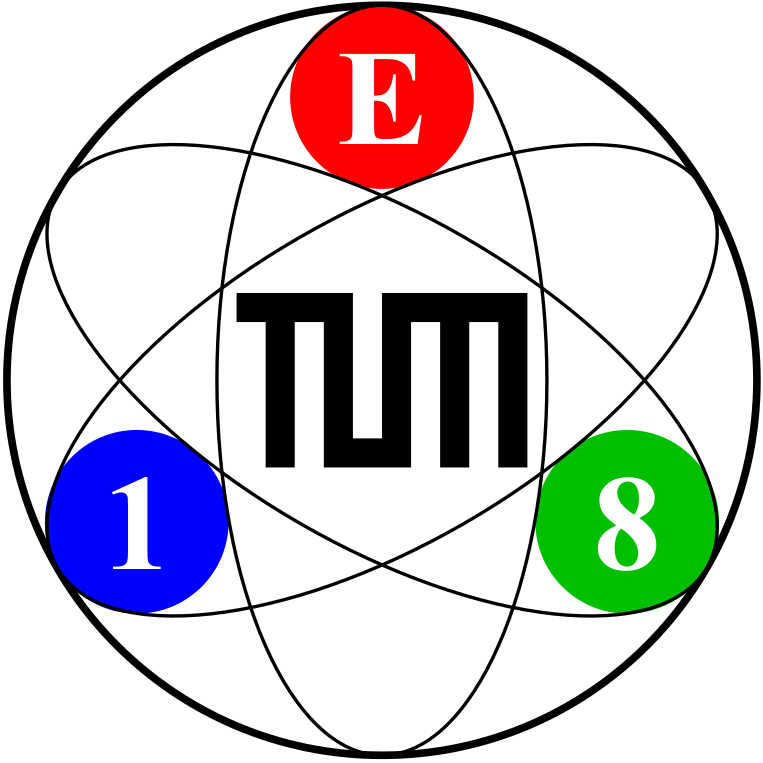
\includegraphics[width=0.8\textwidth]{E18Logo.png}
    \caption{Comparison of the threshold scan of the Citiroc1A ASICs of FPGA 1 and FPGA 2 to a threshold scan performed on a by Weeroc provided testboard.}
    \label{fig:threshold_scan_comparison}
\end{figure}
The pedestal of the threshold scan performed with the frontend electronics is far larger than the pedestal of the threshold scan performed with the by testboard.
This could be due to the fact that the input signals of the Citiroc1A ASICs pick up high frequency signals from the FPGA or the frontend electronics. 
\newline
(INSERT:Place holder for actual results)
\newline
The s-curve analysis shows that the noise of the Citiroc1A ASICs is in the expected range.
\newline
(INSERT:Place holder for actual results)